\subsection{Description des composants}

Nous avons séparé le câblage en trois pôles:
\begin{itemize}
    \item Un pôle Son
    \item Un pôle Vision
    \item Un pôle Moteur
\end{itemize}

\noindent Des $wagos$ sont utilisés pour centraliser le GROUND et les alimentations de la RaspBerry lorsque c'est nécessaire.\\

\large Pôle Son \\
Le premier pôle comprend le système émetteur-récepteur d'ultrasons et le buzzer.
Placé à l'avant, le rôle de ce premier est de calculer la distance qui sépare l'avant du Robot d'un potentiel obstacle.
Si cette distance descend en dessous d'un seuil défini, le Robot doit s'arrêter.
Le buzzer est quand à lui utilisé pour émettre un signal sonore, notament si le Robot s'arrête lorsqu'il rencontre un obstacle.\\

\large Pôle Vision \\
Le deuxième pôle se compose de l'écran LCD, qui est placé sur le dessus du Robot et des trois capteurs de ligne.
Le rôle de l'écran LCD est d'afficher des informations.
Dans le cadre de notre projet, nous l'utilisons pour indiquer les différents ordres que le Robot doit suivre, ainsi que son état d'évolution dans le labyrinthe (lorsqu'il est sorti par exemple).
Nous l'avons également utilisé pour localiser des erreurs lors de nos tests.

Ensuite, les capteurs de ligne sont faits pour envoyer un signal en fonction de la luminosité qu'ils détectent.
C'est le contraste entre les lignes et le reste des tuiles qui les rendent intéressants dans la détection de ligne (comme leur nom l'indique).
Grâce à ces capteurs, nous pouvons détecter les situations dans lesquelles se trouvent le Robot afin qu'il réagisse en conséquence.\\

% Disposition des capteurs (avant = + de marge sur le temps de réaction)
% Quelles combinaisons utiliser pour se repérer 
% Avantage : grande vitesse de réaction, cf video, robot tres efficace
% inconvenient : 1 cas ou le robot bug c'est lorsqu'il se redresse vers une intersection

\large Pôle Moteur \\
Le dernier pôle est bien évidemment dédié aux moteurs.
Ces derniers sont placés à l'arrière du Robot, car c'était à cet emplacement que cela nous paraissait le plus stable, avec une roue ronde à l'avant.
La carte L293D est vissée aux parois du châssis afin de faciliter son accès pour les interventions que nous avons dû faire dessus.

\begin{table}[!h]
    \begin{center}
        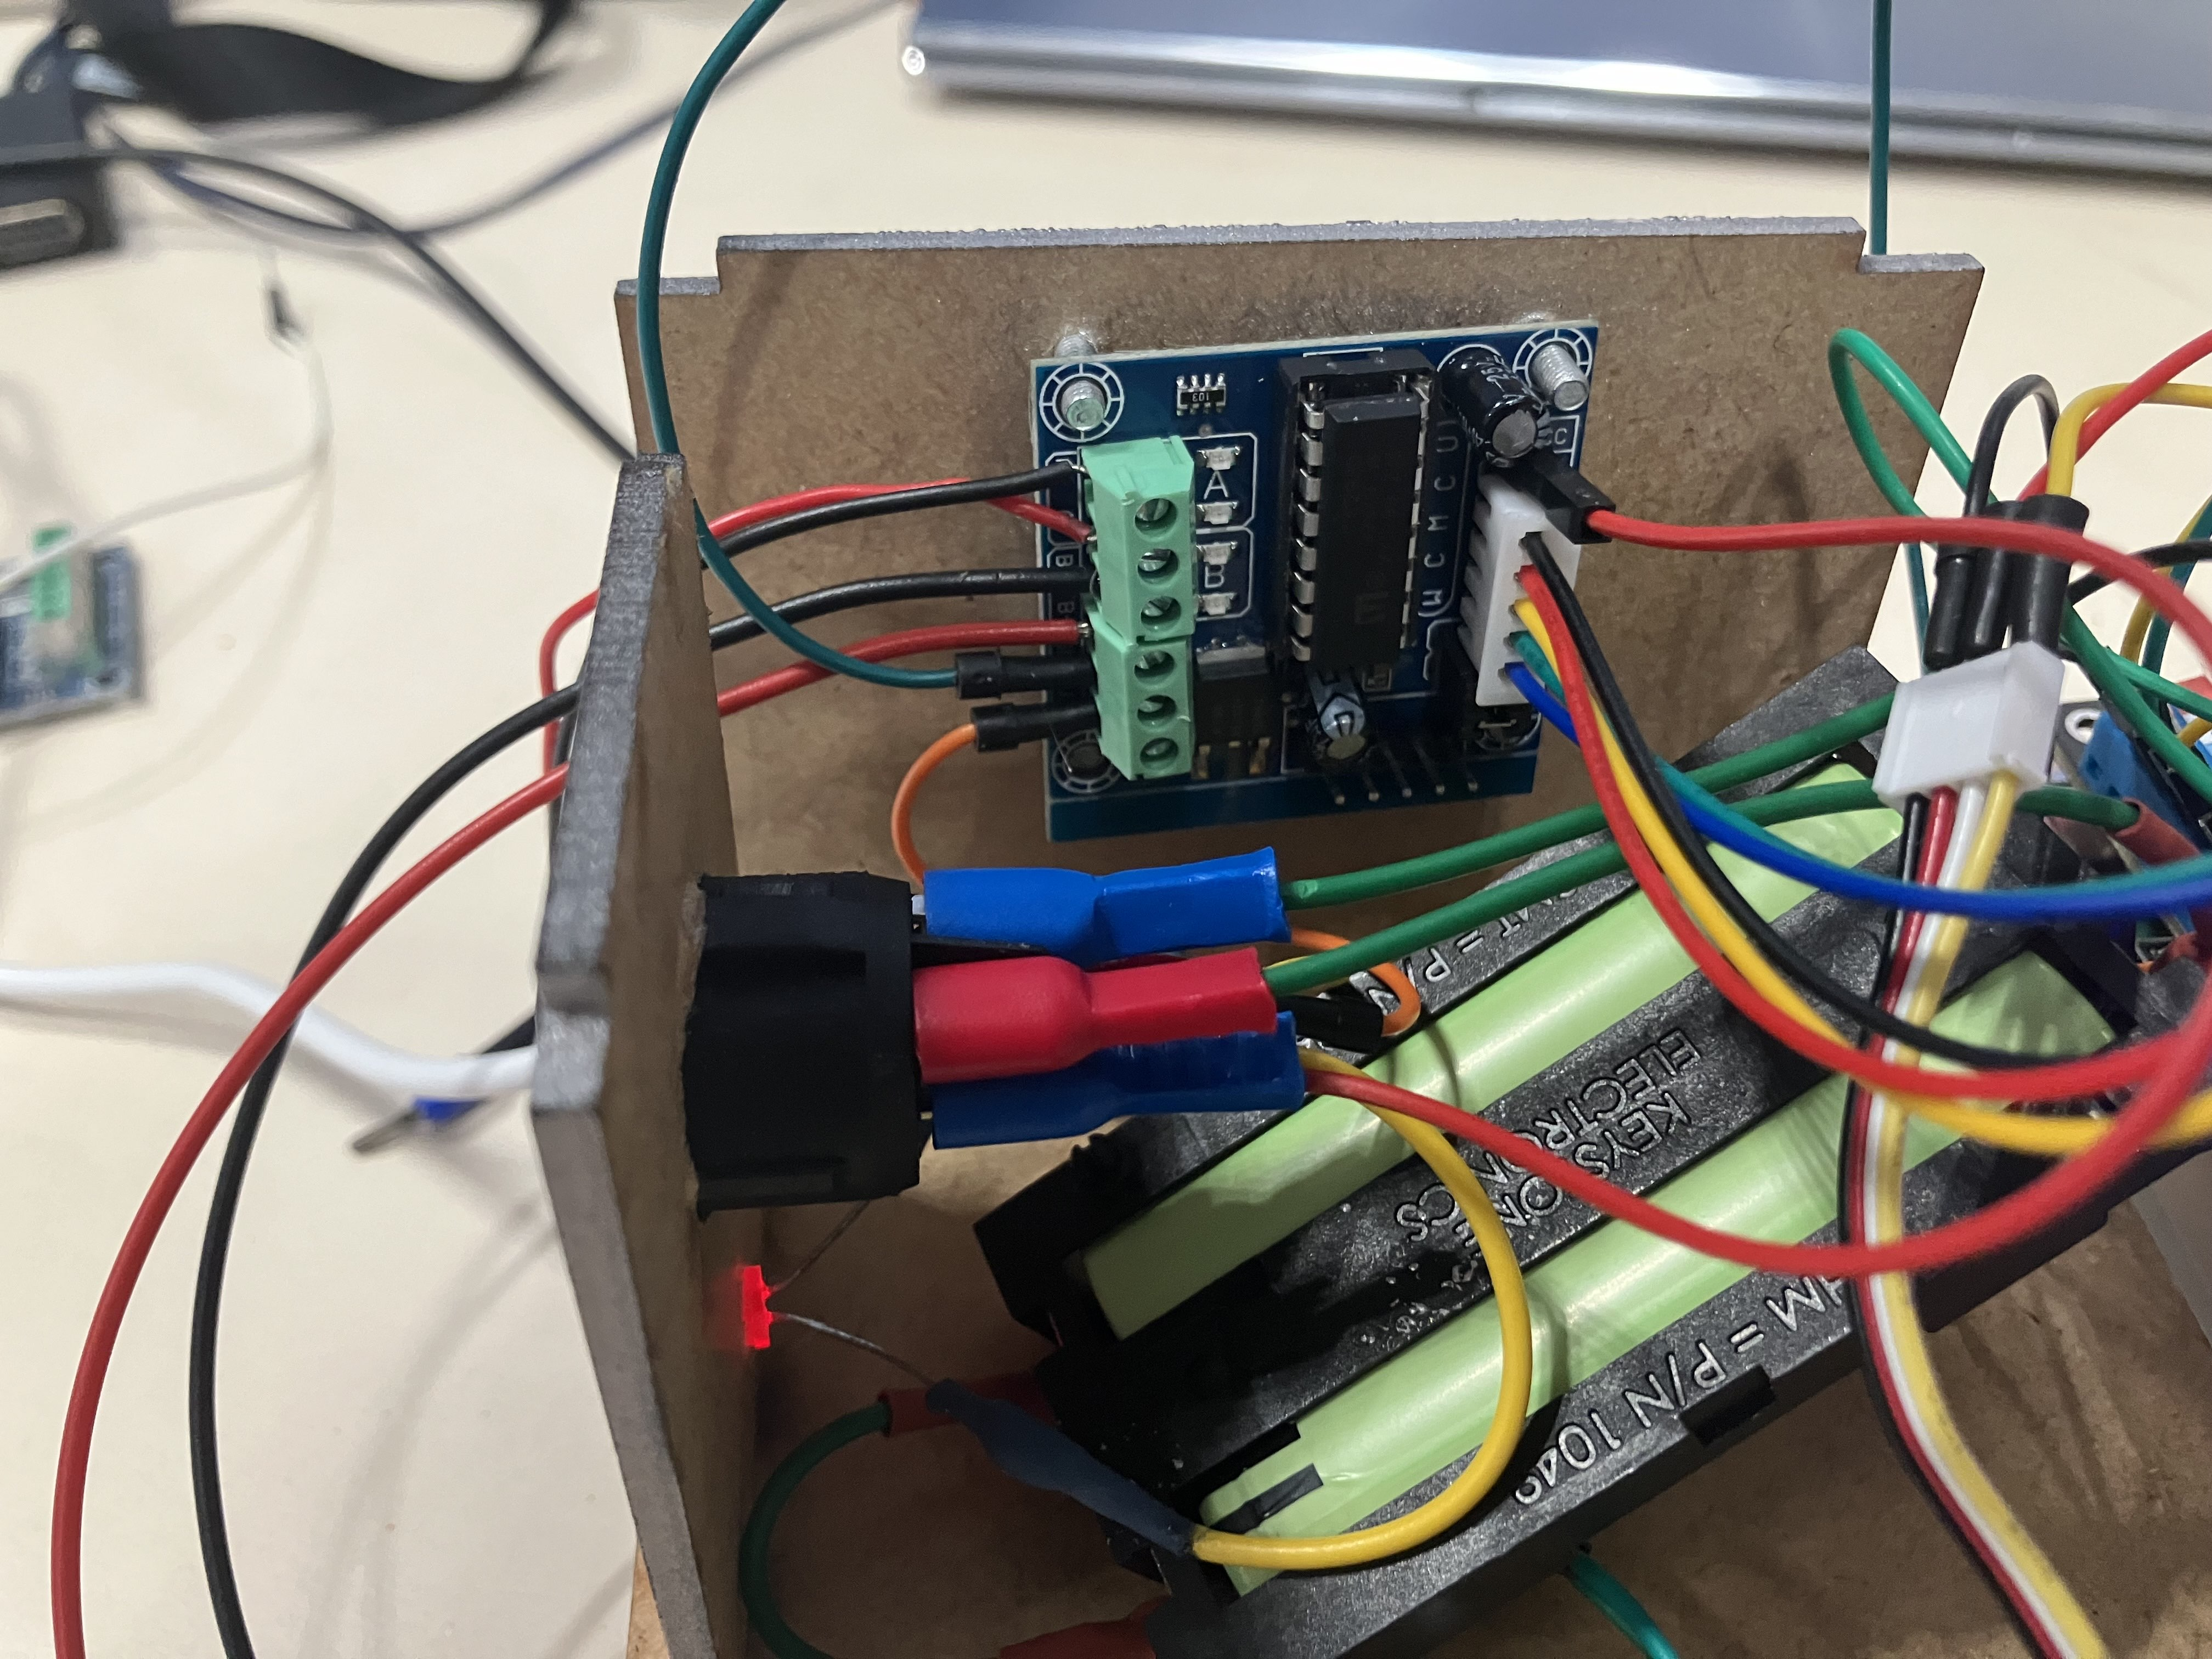
\includegraphics[width = 10cm]{figures/moteursRobot.jpg}
    \end{center}
    \caption{Emplacement des moteurs}
\end{table}

% On nous a demandé de mettre un interrupteur et une LED = protection = resistance
% Pour pas baisser la tension delivrer a la carte et aux moteurs => montage en série
% soudure au niveau du boitier à pile et "pince" pour l'interrupteur


\begin{table}[!h]
    \begin{center}
        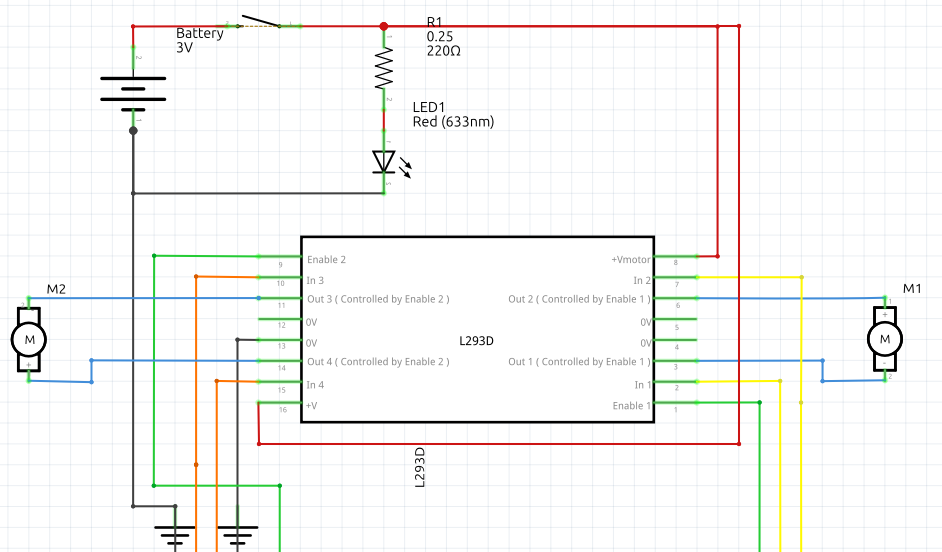
\includegraphics[width = 15cm]{figures/schemaElecMoteurs.png}
        \caption{Schéma électrique du pôle Moteur}     
    \end{center}
\end{table}

\pagebreak